\section{Apéndice: precisión y resumen de las redes}

\begin{figure}[h!]
    \centering
    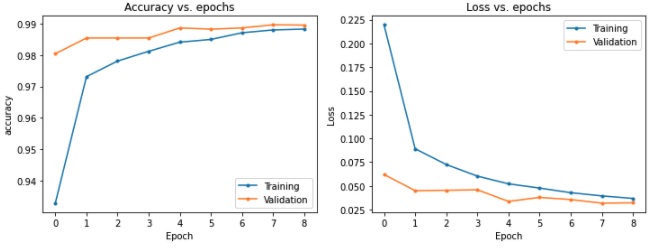
\includegraphics[width=0.85\textwidth]{images/model_details/mnist_linear_good_train.png}
    \caption{Precisión y pérdida de LeNet para MNIST}
    \label{lenet prec}
\end{figure}

\vspace{7mm}

\begin{figure}[h!]
    \centering
    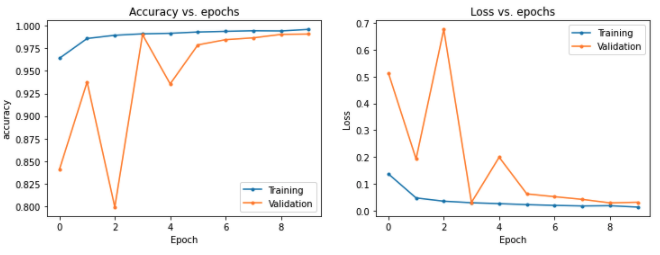
\includegraphics[width=0.85\textwidth]{images/model_details/mnist_nonlinear_good_train.png}
    \caption{Precisión y pérdida de ResNet para MNIST}
    \label{resnet prec}
\end{figure}

\vspace{7mm}

\begin{figure}[h!]
    \centering
    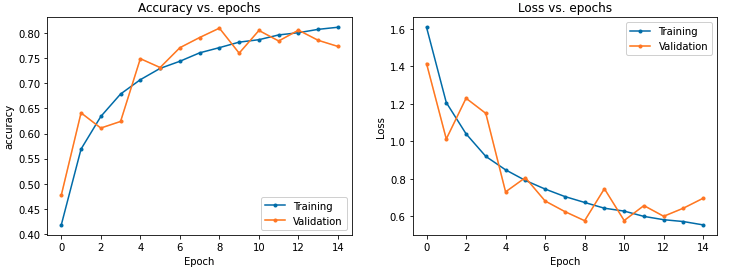
\includegraphics[width=0.85\textwidth]{images/model_details/cifar_train.png}
    \caption{Precisión y pérdida de la red para CIFAR-10}
    \label{cifar prec}
\end{figure}

\begin{figure}[h!]
    \centering
    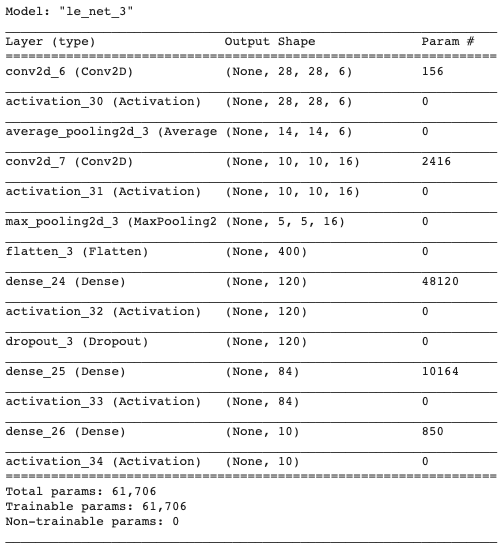
\includegraphics[width=0.65\textwidth]{images/model_details/mnist_linear_good_summary.png}
    \caption{Resumen de LeNet para MNIST}
    \label{lenet summary}
\end{figure}

\begin{figure}[h!]
    \centering
    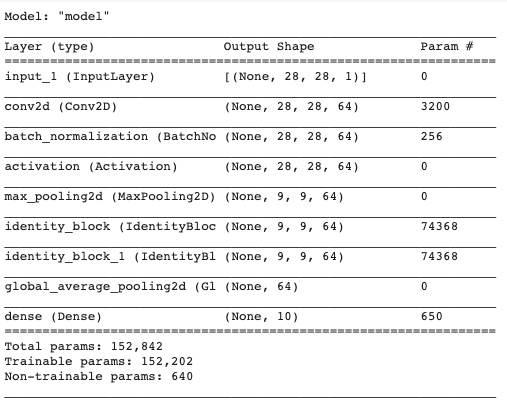
\includegraphics[width=0.65\textwidth]{images/model_details/mnist_nonlinear_good_summary.png}
    \caption{Resumen de ResNet para MNIST}
    \label{resnet summary}
\end{figure}

\begin{figure}[h!]
    \centering
    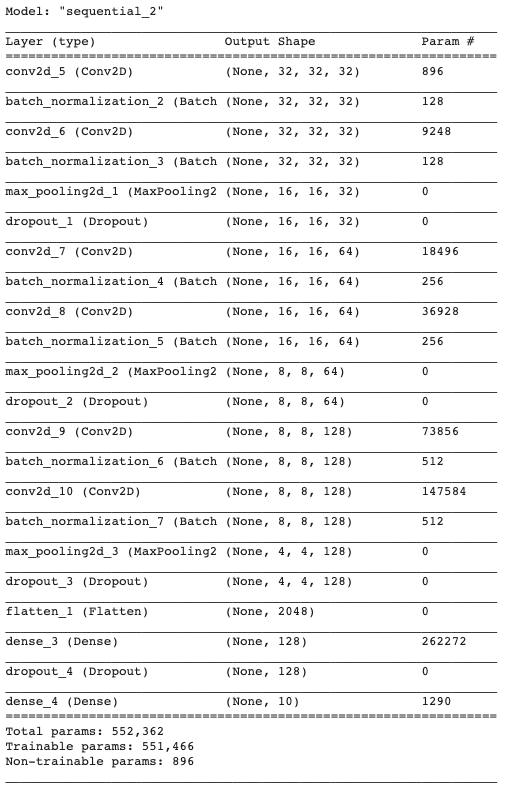
\includegraphics[width=0.75\textwidth]{images/model_details/cifar_summary.png}
    \caption{Resumen de la red específica para CIFAR-10 \cite{cifar_nb}}
    \label{cifar summary}
\end{figure}